
%(BEGIN_QUESTION)
% Copyright 2007, Tony R. Kuphaldt, released under the Creative Commons Attribution License (v 1.0)
% This means you may do almost anything with this work of mine, so long as you give me proper credit

Industrial signal cables are often comprised of {\it twisted, shielded wire pairs}.  Both the twisting of the wire pairs and the shielding encapsulating the pairs works to protect the signals from corruption due to external noise.  One of these techniques guards against interference from stray electrical fields while the other guards against interference from stray magnetic fields.  Identify which does which, and explain why.

$$\includegraphics[width=15.5cm]{i02192x01.eps}$$

Furthermore, explain how a multimeter set to measure AC voltage (ideally, AC millivolts) could be used to detect the presence of {\it electric} field-induced noise anywhere along the cable's length.  Also, explain how a multimeter set to measure AC millivoltage could be used to detect the presence of {\it magnetic} field-induced noise anywhere along the cable's length.

\vskip 20pt \vbox{\hrule \hbox{\strut \vrule{} {\bf Suggestions for Socratic discussion} \vrule} \hrule}

\begin{itemize}
\item{} Identify what would cause a {\it ground loop} to form in this cable, why that would be a bad thing, and how we may avoid it.
\item{} Is the {\it rate of twist} of the wire pair relevant to noise immunity?  If so, which would be better -- a cable with a ``slow'' twist or a cable with a tightly-twisted wire pair?
\end{itemize}

\underbar{file i02192}
%(END_QUESTION)





%(BEGIN_ANSWER)

Shielding guards against electric fields by creating a zero-potential surface around the wires to act as a terminal point for any external electric fields.  Thus, the space inside the cable is free from external electric fields by virtue of the shield.

\vskip 10pt

Twisting the wires ensures that a current loop will never be formed to allow electromagnetic induction from external (changing) magnetic fields.  The following ``thought experiment'' comparing two scenarios proves this conclusively:

$$\includegraphics[width=15.5cm]{i02192x02.eps}$$

\filbreak

Demonstration of how to measure electric field noise voltage:

$$\includegraphics[width=15.5cm]{i02192x04.eps}$$

%(END_ANSWER)





%(BEGIN_NOTES)

Current arrows drawn in the direction of {\it conventional flow}:

$$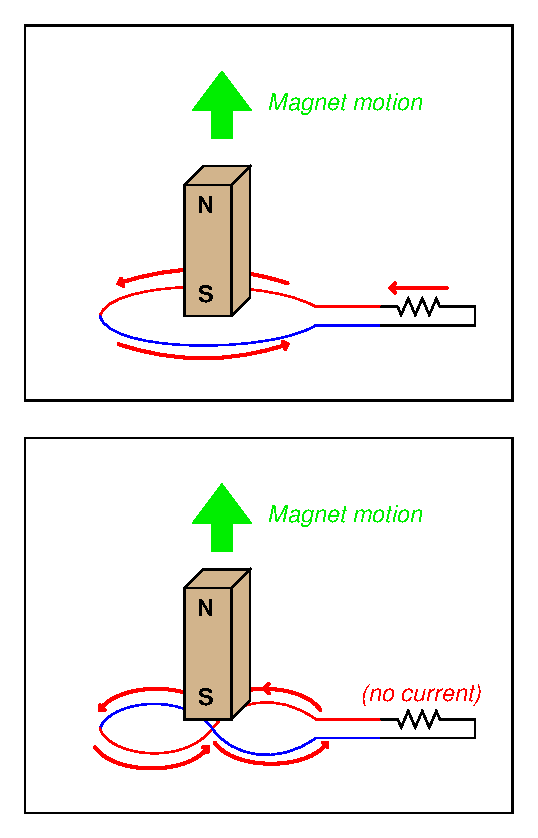
\includegraphics[width=15.5cm]{i02192x03.eps}$$

\filbreak

Demonstration of how to measure magnetic field noise voltage:

$$\includegraphics[width=15.5cm]{i02192x06.eps}$$













\vfil \eject

\noindent
{\bf Prep Quiz:}

The {\it twisting} of conductors and the presence of a {\it shield} in an instrument cable guards against two kinds of interference.  Identify which type of interference is guarded by which feature of the cable:

\begin{itemize}
\item{} Twisting for ground faults; shield for magnetic fields
\vskip 5pt 
\item{} Twisting for magnetic fields; shield for electric fields
\vskip 5pt 
\item{} Twisting for electric fields; shield for physical vibration
\vskip 5pt 
\item{} Twisting for physical vibration; shield for electric fields  
\vskip 5pt 
\item{} Twisting for electric fields; shield for magnetic fields 
\vskip 5pt 
\item{} Twisting for magnetic fields; shield for ground faults 
\end{itemize}


%INDEX% Electronics review: electrical shielding
%INDEX% Electronics review: twisted-pair cable

%(END_NOTES)


